\documentclass[twoside,final]{hcmut-report}

\usepackage[utf8]{inputenc}
\usepackage[T5]{fontenc}
\usepackage[vietnamese]{babel}
\usepackage[protrusion=false]{microtype}

\usepackage{graphicx, caption}
\usepackage{amsmath, extpfeil}
\usepackage{xcolor}
\usepackage{listings}
\usepackage{multirow,multicol}
\usepackage{enumitem}
\usepackage{hyperref}
\usepackage{float}
\usepackage{booktabs}
\usepackage{longtable}
\usepackage{array}
\usepackage{tabularx}
\usepackage{makecell}
\usepackage{subcaption}
\usepackage{tikz}
\usepackage{tkz-tab}
\usepackage{pgfplots}
\usepackage[most]{tcolorbox}
\usepackage{wrapfig}

\AtBeginDocument{\counterwithin{lstlisting}{section}}
\newtcolorbox{exercisebox}{
  enhanced,
  breakable,
  colback=white,
  colframe=black,
  arc=3mm,
  boxrule=0.4pt,
  width=\textwidth,
  left=5pt,
  right=5pt,
  top=5pt,
  bottom=5pt,
  fontupper=\normalsize,
  before upper={\setlength{\parindent}{2em}}
}
\newcommand{\exercise}[1]{\begin{exercisebox}#1\end{exercisebox}}
\newcommand{\result}[1]{\fcolorbox{red}{white}{#1}}
\newcommand{\divides}{\mathrel{\vdots}}
\renewcommand{\cite}[1]{``#1''}
\begin{document}

% \coverpage\clearpage
\tableofcontents\clearpage

\fancyfoot{}
\fancyfoot[L]{\scriptsize \ttfamily Toán 12 - Ltro x doxncwfn - 2526}
\fancyfoot[R]{\scriptsize \ttfamily Trang {\thepage}/\pageref{LastPage}}

\setcounter{page}{1}
\section{Xác suất thống kê}
\subsection{Lý thuyết}
\paragraph*{Định nghĩa}
Cho hai biến cố $A$ và $B$. Xác suất của biến cố $A$ với điều kiện biến cố $B$ đã xảy ra được gọi là xác suất của $A$ với điều kiện $B$, kí hiệu là $P(A | B)$.

Nếu $P(B) > 0$ thì:
\[
    P(A | B) = \frac{P(A \cap B)}{P(B)}.
\]
\paragraph*{Nhận xét}
\begin{itemize}[itemsep=0pt, topsep=0pt, parsep=0pt,label=-]
    \item Từ định nghĩa của xác suất có điều kiện, ta suy ra $P(A \cap B) = P(B) \cdot P(A | B)$.
    \item Người ta chứng minh được rằng
          \[
              \mathrm{P}(A \cap B) = \mathrm{P}(A) \cdot \mathrm{P}(B | A) = \mathrm{P}(B) \cdot \mathrm{P}(A | B).
          \]
          Công thức trên được gọi là công thức nhân xác suất.
    \item Người ta cũng tính $P(A | B) = \dfrac{n(A \cap B)}{n(B)}$.
\end{itemize}
\paragraph*{Công thức xác suất đầy đủ}
Cho 2 biến cố $A$, $B$ với $0 < P(B) < 1$, ta có:
\[
    P(A) = P(A \cap B) + P(A \cap \overline{B}).
\]

Mặt khác:
\begin{align*}
    P(A \cap B)            & = P(B) \cdot P(A | B)                       \\
    P(A \cap \overline{B}) & = P(\overline{B}) \cdot P(A | \overline{B})
\end{align*}

Từ đó ta có công thức xác suất đầy đủ như sau:
\[
    P(A) = P(B) \cdot P(A | B) + P(\overline{B}) \cdot P(A | \overline{B}).
\]
\subsection{Bài toán chia kẹo Euler}
\paragraph*{Phát biểu bài toán} Có $n$ chiếc kẹo và $m$ em nhỏ, có bao nhiêu cách chia kẹo cho các em nhỏ mà mỗi em được nhận ít nhất $1$ chiếc kẹo?
\subsection{Công thức Bayes}
Từ công thức nhân xác suất:
\[
    P(B | A) \cdot P(A) = P(B) \cdot P(A | B) = P(A \cap B).
\]

Với hai biến cố $A, B$ mà $P(A) > 0$, ta có công thức xác suất Bayes:
\[
    P(B | A) = \frac{P(B) \cdot P(A | B)}{P(A)}.
\]

Do \(P(A) = P(B) \cdot P(A | B) + P(\overline{B}) \cdot P(A | \overline{B})\), nên công thức Bayes còn có dạng:
\begin{center}
    \result{$P(B | A) = \dfrac{P(B) \cdot P(A | B)}{P(B) \cdot P(A | B) + P(\overline{B}) \cdot P(A | \overline{B})}$}
\end{center}
\subsection{Xích Markov}
Mô hình Markov là một mô hình xác suất gồm một tập hợp hữu hạn các trạng thái và các xác suất chuyển trạng thái, trong đó xác suất chuyển sang trạng thái tiếp theo chỉ phụ thuộc vào trạng thái hiện tại, phụ thuộc vào 2 yếu tố chính:
\begin{itemize}[itemsep=0pt, topsep=0pt, parsep=0pt,label=-]
    \item Mô hình đầu vào, biểu thị điều kiện hoặc số lượng ban đầu: $I_{m\times 1}$ (Initial State) với $m$ là số lượng tham số.
    \item Mô hình chuyển trạng thái, biểu thị mối liên hệ giữa các đại lượng: $M_{m\times m}$ (Modification), trong đó đại lượng $x_{ab}$ biểu thị mối liên hệ giữa đại lượng $b$ từ đại lượng $a$.
\end{itemize}

Sự chuyển trạng thái giữa 2 lần chuyển đổi liên tiếp nhau được biểu thị: $I_{n} = M\cdot I_{n-1}$\par
Vậy sau khi trải qua $n$ lần chuyển đổi, xác suất của mô hình là: \[\result{$I_{n} = M^n\cdot I_0$}\]
\textbf{Ví dụ}
\exercise{Cuối năm 2036, tiểu vương quốc Mộ Bikini LGBT Skibidi thực hiện khảo sát thống kê thành phần chính trong ngành công nghiệp nặng trọng điểm Scammer, Đố Bạn, Streamer thu được kết quả so với năm trước như sau:
    \begin{itemize}[itemsep=0pt, topsep=0pt, parsep=0pt,label=-]
        \item Mỗi đơn vị đầu ra ngành Scammer cần $(0\%, 30\%, 20\%)$.
        \item Mỗi đơn vị đầu ra ngành Đố Bạn cần $(45\%, 5\%, 5\%)$.
        \item Mỗi đơn vị đầu ra ngành Streamer cần $(35\%, 10\%, 0\%)$.
    \end{itemize}

    Trong đó $(A, B, C)$ là số đơn vị đầu vào của ngành $A$, $B$, $C$. Giả sử số liệu trên không đổi qua các năm, tính cơ cấu kinh tế của mỗi ngành vào năm 2063, biết năm 2036 kim ngạch kinh tế của các ngành lần lượt là $100$, $200$, $120$ triệu USD.
}
Mô hình ma trận đầu vào và ma trận chuyển đổi: $I_0 = \begin{pmatrix}
        100 \\
        200 \\
        120
    \end{pmatrix}$ (triệu USD), $M = \begin{pmatrix}
        0   & 0.45 & 0.35 \\
        0.3 & 0.05 & 0.1  \\
        0.2 & 0.05 & 0
    \end{pmatrix}$

$\Rightarrow I_{27} = M^{27}\cdot I_0 = \begin{pmatrix}
        0   & 0.45 & 0.35 \\
        0.3 & 0.05 & 0.1  \\
        0.2 & 0.05 & 0
    \end{pmatrix}^{27} \times \begin{pmatrix}
        100 \\
        200 \\
        120
    \end{pmatrix} = \begin{pmatrix}
        2.000\cdot 10^{-4} \\
        1.518\cdot 10^{-4} \\
        9.380\cdot 10^{-4}
    \end{pmatrix}$

Vậy Scammer, Đố Bạn, Streamer chiếm lần lượt $2.000\cdot 10^{-6}\%$, $1.518\cdot 10^{-6}\%$, $9.380\cdot 10^{-6}\%$ cơ cấu kinh tế.
\subsection{Bài tập}
\exercise{Theo một số liệu thống kê, năm 2004 ở Canada có 65\% nam giới là thừa cân và 53,4\% nữ giới là thừa cân. Nam giới và nữ giới ở Canada đều chiếm 50\% dân số cả nước. Hỏi trong năm 2004, xác suất để một người Canada được chọn ngẫu nhiên là người thừa cân bằng bao nhiêu?}

Xét hai biến cố:
\begin{itemize}[itemsep=0pt, topsep=0pt, parsep=0pt,label=-]
    \item $A$: ``Người được chọn ra là người thừa cân'';
    \item $B$: ``Người được chọn ra là nam giới'' $\Rightarrow\overline{B}$: ``Người được chọn ra là nữ giới''.
\end{itemize}

Từ giả thiết:
$\begin{cases}
        \mathrm{P}(B) = \mathrm{P}(\overline{B}) = 50\% = 0{,}5 \\
        \mathrm{P}(A | B) = 65\% = 0{,}65                       \\
        \mathrm{P}(A | \overline{B}) = 53.4\% = 0{,}534.
    \end{cases}$

Theo công thức xác suất toàn phần:
\[
    \mathrm{P}(A) = \mathrm{P}(B) \cdot \mathrm{P}(A | B) + \mathrm{P}(\overline{B}) \cdot \mathrm{P}(A | \overline{B})
    = 0.5 \cdot 0.65 + 0.5 \cdot 0.534 = \result{0.592}.
\]
\exercise{Một hộp chứa 9 thẻ được đánh số từ 1 tới 9, bạn A lấy ngẫu nhiên 1 thẻ từ hộp, xem rồi bỏ ra ngoài. Nếu thẻ là số chẵn thì A cho vào hộp 2 số 10 và 11. Nếu thẻ là số lẻ thì A cho thêm vào số 12, 13, 14. Bạn B lấy 3 thẻ ngẫu nhiên từ hộp. Gọi X là tích các số trên thẻ B lấy ra, biết X chia hết cho 2, tính xác suất của bạn A lấy ra được số chẵn.
}
\begin{wrapfigure}{r}{0.25\textwidth}
    \centering
    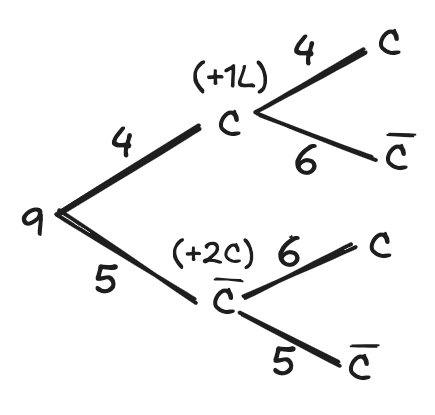
\includegraphics[width=1.2\linewidth]{images/XSTK/2.png}
\end{wrapfigure}
Gọi $C$ là biến cố lấy được số chẵn.\par
Ta có:
$\begin{cases}
        P(C)\cdot P(X\divides 2|C) = \dfrac{4}{9}\cdot(1-\dfrac{C_6^3}{\displaystyle C_{10}^3}) \\
        P(\overline{C})\cdot P(X\divides 2|\overline{C}) = \dfrac{5}{9}\cdot(1-\dfrac{C_5^3}{\displaystyle C_{11}^3})
    \end{cases}$\par
$\Rightarrow P(C|X\divides 2) = \dfrac{\dfrac{4}{9}\cdot(1-\dfrac{C_6^3}{\displaystyle C_{10}^3})}{\dfrac{4}{9}\cdot(1-\dfrac{C_6^3}{\displaystyle C_{10}^3}) + \dfrac{5}{9}\cdot(1-\dfrac{C_5^3}{\displaystyle C_{11}^3})} =\dfrac{572}{1351}\approx \result{0.4151}$
\subsection{Đề thi thử trường sở}
\exercise{\textcolor{red}{\textit{2425 -- Sở GDĐT Nghệ An -- Đợt 3}}

    \begin{wrapfigure}{r}{0.17\textwidth}
        \centering
        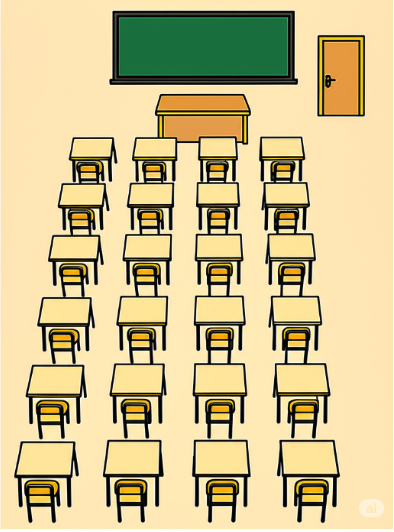
\includegraphics[width=1.08\linewidth]{images/Nghệ An 2025 - Đợt 3/NgheAn25-2.png}
    \end{wrapfigure}
    Cúm A (Influenza A) là bệnh nhiễm trùng đường hô hấp cấp tính do các virus cúm mùa gây nên. Virus cúm A có thể lây truyền trực tiếp trong không khí thông qua đường hô hấp. Giả sử Virut cúm A có khả năng lấy nhiễm đối với người ngồi trong vòng bán kính $1,9m$ là $85\%$ và đối với người ngồi cách hơn $1,9m$ là $5\%$. An là một học sinh bị nhiễm cúm A nhưng bản thân không hay biết. An đi dự thi cuối kỳ. Phòng thi của An có $24$ bạn được xếp vào $24$ chỗ ngồi của một phòng thi có $4$ dãy, mỗi dãy $6$ chỗ ngồi như hình vẽ. Khoảng cách giữa hai người theo hàng ngang là $1,6m$, theo hàng dọc là 1m (hình vẽ). Do không biết trước An bị cúm A nên các thí sinh được xếp ngẫu nhiên vào phòng thi. Một bạn cùng phòng của An sau khi dự thi đi kiểm tra thấy không bị nhiễm cúm. Tính xác suất để thí sinh đó ngồi gần An trong vòng $1,9m$. \textit{(Làm tròn kết quả đến hàng phần trăm)}.
}
\begin{wrapfigure}{r}{0.25\textwidth}
    \centering
    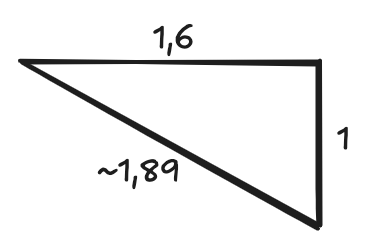
\includegraphics[width=0.8\linewidth]{images/Nghệ An 2025 - Đợt 3/NgheAn25-3.png}
    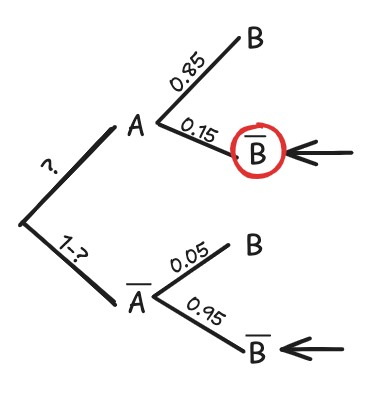
\includegraphics[width=1.2\linewidth]{images/Nghệ An 2025 - Đợt 3/NgheAn25-4.png}
\end{wrapfigure}

Gọi $A$ là biến cố ngồi gần An, $B$ là biến cố bị nhiễm bệnh.\par
Vì nếu ngồi chéo An thì bạn đó vẫn bị nhiễm bệnh nên xét vị trí An được xếp:
\begin{itemize}[itemsep=0pt, topsep=0pt, parsep=0pt,label=-]
    \item Nếu An ngồi ở 1 trong 4 góc phòng, chỉ có $3$ vị trí trong bán kính lây bệnh.
    \item Nếu An ngồi ở 1 trong 12 rìa phòng, có $5$ vị trí trong bán kính lây bệnh.
    \item Nếu An ngồi ở 1 trong 8 vị trí giữa phòng, có $8$ vị trí trong bán kính lây bệnh.
\end{itemize}

$\Rightarrow P(A) = \dfrac{4}{24}\cdot\dfrac{3}{23} + \dfrac{12}{24}\cdot\dfrac{5}{23} + \dfrac{8}{24}\cdot\dfrac{8}{23} = \dfrac{17}{69} \Rightarrow P(\overline{A}) = \dfrac{52}{69}$\\
$\Rightarrow P(A|\overline{B}) = \dfrac{\dfrac{17}{69}\cdot 0.15}{\dfrac{17}{69}\cdot 0.15 + \dfrac{52}{69}\cdot0.95} \approx 0.0491 \approx$ \result{$0.05$}

\exercise{\textcolor{orange}{\textit{2425 -- Sở GDĐT Nghệ An -- Đợt 3}}

    Một nghiên cứu dịch tễ học trong một cộng đồng dân số tại một địa phương X đưa ra các số liệu sau:
    \begin{itemize}[itemsep=0pt, topsep=0pt, parsep=0pt,label=-]
        \item Tỷ lệ người có hút thuốc lá là 25\%.
        \item Tỷ lệ bị ung thư phổi ở nhóm người hút thuốc lá là 2\%, trong khi ở nhóm người không hút thuốc lá chỉ là 0,1\%.
    \end{itemize}

    Xét một người được chọn ngẫu nhiên từ cộng đồng này. Ký hiệu $A$ là biến cố ''Người đó bị ung thư phổi'' và $B$ là biến cố ''Người đó có hút thuốc lá''.
    \begin{enumerate}[itemsep=0pt, topsep=0pt, parsep=0pt,label=\alph*)]
        \item $P(A|B) = 0,1$
        \item Nếu một người bị ung thư phổi, thì xác suất người đó có hút thuốc lá là 0,8 (làm tròn đến hàng phần mười).
        \item Tỷ lệ người bị ung thư phổi ở địa phương X là 1,5\%
        \item Dựa trên các số liệu này, tỷ lệ người bị ung thư phổi ở nhóm người có hút thuốc lá cao gấp 20 lần so với ở nhóm người không hút thuốc.
    \end{enumerate}}
\begin{minipage}{0.35\textwidth}
    \begin{figure}[H]
        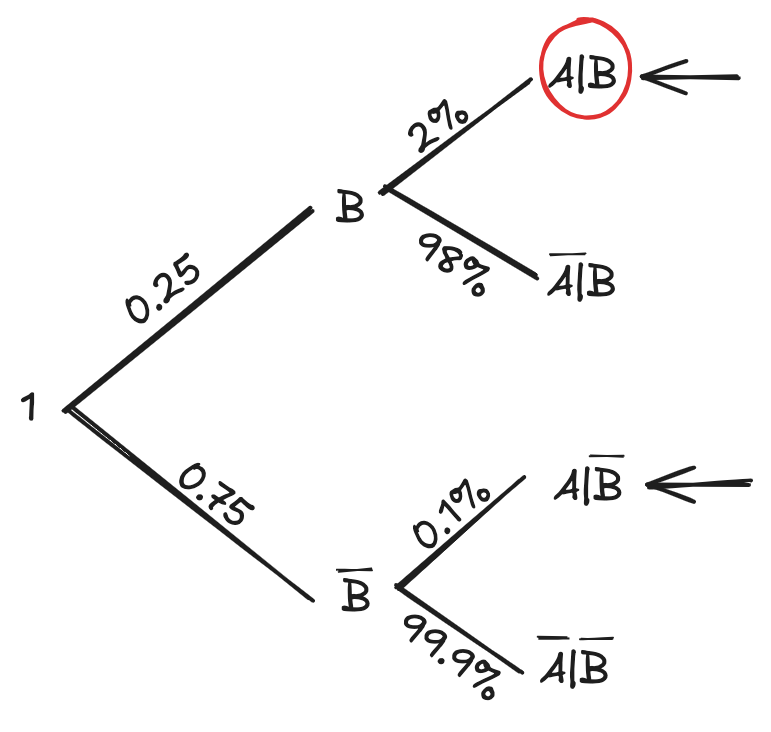
\includegraphics[width=\textwidth]{images/Nghệ An 2025 - Đợt 3/NgheAn25-1.png}
    \end{figure}
\end{minipage}
\begin{minipage}{0.65\textwidth}
    a) Từ đề bài: $\begin{cases}
            \result{P(A|B)=2\%}       \\
            P(A|\overline{B}) = 0,1\% \\
            P(B) = 0.25
        \end{cases} \Rightarrow$ \textcolor{red}{Sai}\\

    b) $P(A|B) = \dfrac{2\%\cdot 0.25}{2\%\cdot 0.25 + 0.75\cdot 0.1\%} \approx \result{0.9} \Rightarrow$ \textcolor{red}{Sai}\\

    c) $P(A) = 2\%\cdot 0.25 + 0.1\%\cdot 0.75 = \result{5.75\%} \Rightarrow$ \textcolor{red}{Sai}\\

    d) $\dfrac{P(A|B)}{P(A|\overline{B})} = \dfrac{2\%}{0.1\%} = \result{20}\Rightarrow$  \textcolor{red}{Đúng}
\end{minipage}

\exercise{
    \textcolor{orange}{\textit{2425 -- Cụm trường Tuyên Quang - Vĩnh Phúc}}

    Ông Hùng hằng ngày đi làm bằng xe máy hoặc xe buýt. Tỉ lệ trễ giờ nếu ông đi làm bằng xe máy là $5\%$, bằng xe buýt là $10\%$. Xét trong tháng 6, ông Hùng ngày nào cũng đi làm đều đặn và trong ngày đầu tiên của tháng, xác suất ông chọn đi làm bằng xe máy là $60\%$.

    Từ ngày thứ hai trở đi, cách ông Hùng chọn phương tiện đi làm phụ thuộc vào việc ông có bị trễ giờ trong ngày hôm trước hay không:
    \begin{itemize}[itemsep=0pt, topsep=0pt, parsep=0pt,label=-]
        \item Nếu ngày hôm trước ông Hùng không bị trễ giờ thì ông ấy tiếp tục sử dụng loại phương tiện mà ông đã đi trong ngày hôm trước.
        \item Nếu ngày hôm trước ông Hùng bị trễ giờ thì ông sẽ chuyển sang sử dụng loại phương tiện còn lại.
    \end{itemize}
    ,
    Xác suất để ngày cuối cùng của tháng 6 ông Hùng đi làm bằng xe máy là $p$, khi đó giá trị của $10^4\cdot p$ là? \textit{(kết quả làm tròn đến hàng đơn vị)}
}
\begin{figure}[H]
    \centering
    \includegraphics*[width=0.35\textwidth]{images/XSTK/TQ-VP.png}
\end{figure}
Áp dụng mô hình Markov: $I_{30} = M^{29}\cdot I_1 = \begin{pmatrix}
        0.95 & 0.9 \\
        0.05 & 0.1
    \end{pmatrix}^{29} \begin{pmatrix}
        0.6 \\ 0.4
    \end{pmatrix} \approx \begin{pmatrix}
        0.6661 \\0.3339
    \end{pmatrix} \Rightarrow \result{$10^4\cdot p = 6661$}$

\exercise{
    \textcolor{orange}{\textit{2425 -- THPT Tĩnh Gia 1 - Thanh Hoá}}

    Có hai chiếc hộp, hộp $I$ có $6$ quả bóng màu đỏ và một số quả bóng màu xanh, hộp $II$ có $7$ quả bóng màu đỏ và $3$ quả bóng màu xanh, các quả bóng có cùng kích thước và khối lượng. Lấy ngẫu nhiên một quả bóng từ hộp $I$ bỏ vào hộp $II$. Sau đó, lấy ra ngẫu nhiên hai quả bóng từ hộp $II$. Xác suất lấy được ít nhất một quả bóng đỏ từ hộp $II$ bằng $\dfrac{32}{35}$. Tính xác suất để quả bóng được lấy ra từ hộp $I$ là quả bóng đỏ, biết rằng hai quả bóng lấy ra từ hộp $II$ có ít nhất một quả bóng đỏ. \textit{(làm tròn kết quả đến hàng phần trăm)}}

Gọi $n$ là số quả bóng xanh ở hộp I. ($n\in\mathbb{N}^*$)\par
Gọi $A$ là biến cố ''quả bóng lấy được ở hộp I là bóng đỏ''
$\Rightarrow \begin{cases}
        P(A) = \dfrac{6}{n+6} \\
        P(\overline{A}) = \dfrac{n}{n+6}
    \end{cases}$\par
Gọi $B$ là biến cố ''hai quả bóng lấy ra từ hộp II là có ít nhất một quả bóng đỏ''\par
$\Rightarrow P(\overline{B}|A) = \dfrac{\displaystyle C^2_3}{\displaystyle C^2_{11}} = \dfrac{3}{55}$, $P(\overline{B}|\overline{A}) = \dfrac{\displaystyle C^2_4}{\displaystyle C^2_{11}} = \dfrac{6}{55}$\par
$\Rightarrow P(B) = P(A)\cdot P(B|A) + P(\overline{A})\cdot P(B|\overline{A}) = \dfrac{312 + 49n}{55(n+6)} = \dfrac{32}{35} \Leftrightarrow n = 8$\par
$\Rightarrow P(A|B) = \dfrac{P(A)\cdot P(B|A)}{P(B)} = \dfrac{P(A)\cdot (1 - P(\overline{B}|A))}{P(B)} = \dfrac{\dfrac{6}{14}\cdot(1-\dfrac{3}{55})}{\dfrac{32}{35}} = \dfrac{39}{88} \approx \result{0.44}$\par
\exercise{
    \textcolor{red}{\textit{2425 -- THPT Quỳ Hợp 2 Nghệ An -- Lần 5}}

    Một cơ sở sản xuất sữa giả mua các thùng sữa thật giống nhau ($48$ hộp/thùng), rồi thay thế một số hộp sữa thật thành các hộp sữa giả nhằm thu lợi bất chính. Trong quá trình sản xuất, cơ sở phân ra làm $2$ loại: loại $I$ để lẫn mỗi thùng $5$ hộp sữa giả và loại $II$ để lẫn mỗi thùng $3$ hộp sữa giả. Biết rằng số thùng sữa loại $I$ bằng $1.5$ lần số thùng sữa loại $II$. Chọn ngẫu nhiên 1 thùng sữa từ cơ sở sản xuất và từ thùng đó lấy ra ngẫu nhiên $10$ hộp. Tính xác suất để trong $10$ hộp lấy ra có đúng $2$ hộp sữa là giả \textit{(làm tròn kết quả đến hàng phần trăm)}.}
Gọi $A$ là biến cố ``thùng sữa được chọn thuộc loại $I$'' $\Rightarrow \begin{cases}
        P(A) = \dfrac{1.5x}{1.5x + x} \\
        P(\overline{A}) = 1 - P(A)
    \end{cases}$.\par
Gọi $B$ là biến cố ``10 hộp sữa được chọn có 2 hộp sữa giả'' $\Rightarrow \begin{cases}
        P(B|A) = \dfrac{\displaystyle C^2_{5}\cdot C^{8}_{43}}{\displaystyle C^{10}_{48}} \\
        P(B|\overline{A}) = \dfrac{\displaystyle C^2_{3}\cdot C^{8}_{45}}{\displaystyle C^{10}_{48}}
    \end{cases}$.\par
$\Rightarrow P(B) = P(A)\cdot P(B|A) + P(\overline{A})\cdot P(B|\overline{A}) = \dfrac{2052}{11891} \approx \result{$0.17$}$
\exercise{
    \textcolor{red}{\textit{2425 -- THPTQG -- Mã đề 0122}}

    Có $4$ ngăn trong một giá để sách được đánh số thứ tự 1, 2, 3, 4 và $8$ quyển sách khác nhau. Bạn Đặng Cao Bồ xếp hết $8$ quyển sách trên vào $4$ ngăn đó sao cho mỗi ngăn có ít nhất $1$ quyển sách và các quyển sách được xếp thẳng đứng thành một hàng ngang với gáy sách quay ra ngoài ở mỗi ngăn. Thấy vậy, bạn Tá Selu đố bạn Đặng Cao Bồ xem có tất cả bao nhiêu $T$ cách xếp, nếu đoán đúng, bạn Đặng Cao Bồ sẽ scam nóng $\dfrac{T}{600}$\$. Hãy tính giúp bạn Tá Selu số tiền trên biết $2$ cách xếp của bạn Tá Selu được xem là giống nhau nếu chúng thoả mãn đồng thời cả hai điều kiện:
    \begin{itemize}[itemsep=0pt, topsep=0pt, parsep=0pt,label=--]
        \item Với từng ngăn, số lượng quyển sách ở ngăn đó là như nhau trong cả hai cách xếp.
        \item Với từng ngăn, số thứ tự từ trái sang phải của các quyển sách được xếp là như nhau trong cả hai cách xếp.
    \end{itemize}
}
Áp dụng bài toán chia kẹo Euler: $T = 8!\cdot\displaystyle C^3_7 = 1411200 \Rightarrow \dfrac{T}{600} = \result{$2352\$$}$
\newpage\section{Ứng dụng tích phân}
\exercise{
    \textcolor{red}{\textit{2425 -- Sở GDĐT Nghệ An -- Đợt 3}}

    \begin{wrapfigure}{r}{0.35\textwidth}
        \centering
        \includegraphics*[width=1.03\linewidth]{images/Nghệ An 2025 - Đợt 3/NgheAn25-5.png}
    \end{wrapfigure}

    Một lập trình viên tạo một trò chơi. Trong trò chơi đó có một vùng đất hình chữ nhật $ABCD$. Một con sông nằm bên cạnh vùng đất đó, $AD$ là bờ sông. Một giếng nước khoan được đặt tại điểm $I$ nằm trong hình chữ nhật, với:
    $AB = 80$m, $AD = 40$m. Điểm $I$ cách cạnh $AB$ $20$m, cách cạnh $AD$ $60$m. Nhân vật trong game khi đến vùng đất này cần phải di chuyển đến giếng nước hoặc bờ sông để lấy nước.

    Lập trình viên muốn tô màu một phần của vùng đất đó sao cho khi đứng trong vùng tô màu này, nhân vật di chuyển đến giếng nước để lấy nước nhanh hơn so với đến bờ sông.

    Diện tích vùng tô màu đó là bao nhiêu mét vuông? (Giả sử rằng khi di chuyển, vận tốc của nhân vật không đổi; làm tròn kết quả đến hàng đơn vị).
}
\begin{figure}[H]
    \centering
    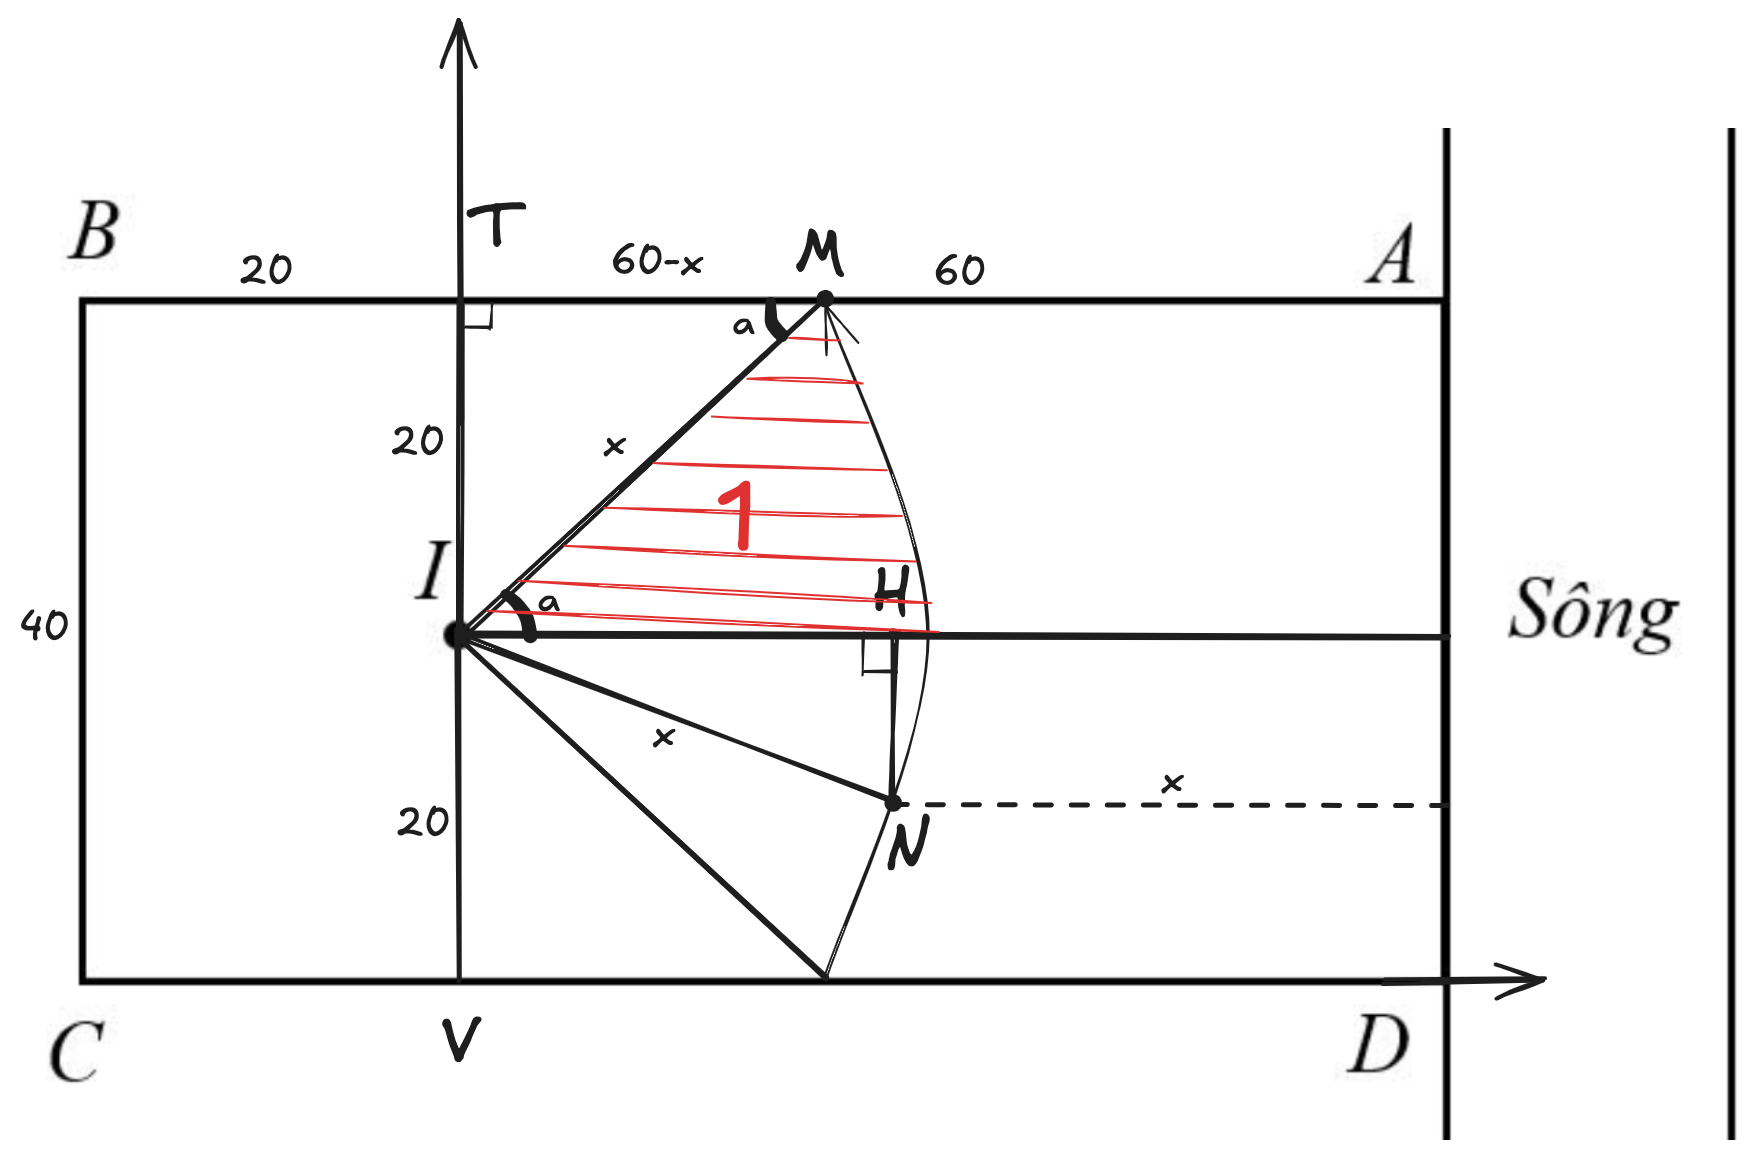
\includegraphics[width=0.6\textwidth]{images/Nghệ An 2025 - Đợt 3/NgheAn25-6.png}
\end{figure}
Khai thác dữ kiện, dễ thấy ranh giới cần tìm có dạng parabolic và ta có số liệu như hình vẽ.\par
Xét $\triangle TIM$: $x^2 = 20^2 + (60-x)^2 \Leftrightarrow x = \dfrac{100}{3}$(m)\par
$\Rightarrow \sin\alpha = \dfrac{20}{100/3} = \dfrac{3}{5} \Rightarrow\alpha=\arcsin(\dfrac{3}{5})$\par
Xét $\triangle IHN$: $IN = \dfrac{IH}{\cos\alpha} = \dfrac{60 - IN}{\cos\alpha} \Leftrightarrow IN = \dfrac{60}{\cos\alpha + 1}$\par
$S = S_{BCVT} + 2S_{\triangle ITM} + 2S_1 = 40\cdot 20 + 2\cdot\dfrac{1}{2}\cdot 20\cdot(60-\dfrac{100}{3}) + 2\cdot\dfrac{1}{2}\displaystyle\int_{0}^{\alpha}(\dfrac{60}{\cos\alpha + 1})^2\,dx$\par
\hspace*{1em}$= \dfrac{17600}{9} \approx$ \result{$1956(m^2)$}

\exercise{
    \textcolor{blue}{\textit{2425 -- Cụm trường Tuyên Quang - Vĩnh Phúc}}

    \begin{wrapfigure}{r}{0.35\textwidth}
        \centering
        \includegraphics*[width=1.03\linewidth]{images/XSTK/TQ-VP-2.png}
    \end{wrapfigure}

    Bác Bình muốn nhờ thợ trang trí một bức tường hình chữ nhật $ADEF$ với kích thước $EF = 6\,\text{m}$, $DE = 3\,\text{m}$ sao cho cân xứng hai nửa. Phần gạch chéo là hình giới hạn bởi đường gấp khúc $AFED$ và nửa đường tròn đường kính $AD$, được thuê sơn với đơn giá 250.000đ/m$^2$. Phần màu trắng giới hạn bởi nửa đường tròn đường kính $AD$ và một đường parabol (có đỉnh $H$ cách đường thẳng $AB$ một khoảng bằng $2\,\text{m}$ và đi qua hai điểm $B, C$ nằm trên cạnh $AD$ thỏa mãn $AB = 1.5\,\text{m}$, $CD = 1.5\,\text{m}$) được thuê trang trí bằng bức phù điêu đắp bằng xi măng với đơn giá 1.950.000đ/m$^2$ (tham khảo hình vẽ).

    Hỏi Bác Bình phải trả bao nhiêu triệu đồng để trang trí bức tường như vậy? (Kết quả làm tròn đến hàng phần mười của triệu đồng)
}
\textit{Cách 1}: Dễ thấy parabola có phương trình $y = -\dfrac{8}{9}x^2 + 2 \Rightarrow S_{(P)} = \displaystyle \int_{-1.5}^{1.5}(-\dfrac{8}{9}x^2 + 2)dx = 4$ (m$^2$)\par
\textit{Cách 2}: $S_{(P)} = \dfrac{2}{3}dh = \dfrac{2}{3}\cdot 3\cdot 2 = 4$ (m$^2$)\par
$S_1 + S_2 = S_{ADEF} - \dfrac{1}{2}S_{(O; OD)} = 3\cdot 6 - \dfrac{1}{2}\pi\cdot 3^2 = 18 - \dfrac{9}{2}\pi$ (m$^2$)\par
$\Rightarrow T = 0.25\cdot(18 - \dfrac{9}{2}\pi) + 1.95\cdot (\dfrac{1}{2}\pi\cdot 3^2 - 4) = \dfrac{3(51\pi-22)}{20} \approx \result{20.7}$ (triệu đồng)

\exercise{
    \textcolor{orange}{\textit{2425 -- Tư duy mở 42}}

    \begin{wrapfigure}{r}{0.2\textwidth}
        \centering
        \includegraphics*[width=1.05\linewidth]{images/Ứng dụng tích phân/TDM42.png}
    \end{wrapfigure}
    Trên mặt phẳng cho hình vuông $ABCD$ có cạnh bằng $60cm$ và một đường parabol $(P)$ như hình vẽ. Gọi $M$ là điểm nằm trên cạnh $BC$ sao cho $BM > CM$ và di chuyển đến $B$ với tốc độ không đổi $2cm/s$. Hãy xác đinh tốc độ thay đổi của diện tích $S$ giới hạn bởi đoạn $AM$ và $(P)$ theo đơn vị $dm^2/s$ ở thời điểm $M$ là trung điểm của cạnh $BC$. \textit{(làm tròn kết quả đến hàng phần mười)}}

Ta có:
$\begin{cases}
        C(30; 60), D(-30;60)\in (P) \Rightarrow (P):y=\dfrac{x^2}{15} \\
        M(30; 60 - 2t) \Rightarrow (d_{AM}):y=(-\dfrac{t}{30}+1)x + (30-t)
    \end{cases}$\par
$\Rightarrow \dfrac{x^2}{15} = (-\dfrac{t}{30}+1)x + (30-t) \Leftrightarrow 2x^2 + (t - 30)x + 30t - 30^2 = 0 \xRightarrow{\text{Viète}}\begin{cases}
        x_1 + x_2 =\dfrac{30-t}{2}  \\
        x_1x_2 =\dfrac{30t-30^2}{2} \\
        x_2 - x_1 =\dfrac{\sqrt{\Delta}}{a}
    \end{cases}$\par
$\Rightarrow S(t) = \displaystyle \int_{x_1}^{x_2}\dfrac{x^2}{15}dx = \left. \frac{x^3}{45} \right|_{x_1}^{x_2} = \dfrac{1}{45}(x_2^3 - x_1^3) = \dfrac{1}{45}(x_2-x_1)(S^2 - P) \Rightarrow S'(15) \overset{\text{Casio}}{\approx} \result{$-0.2\,(dm^2/s)$}$
\exercise{
    \textcolor{blue}{\textit{2425 -- THPT Quỳ Hợp 2 Nghệ An -- Lần 5}}

    Một người thợ gốm sứ muốn tạo ra một sản phẩm là bình sứ tráng men vẽ hoa văn bằng vàng 24K mang ý nghĩa phong thủy \cite{Thuận buồm xuôi gió} như hình vẽ mô tả. Để tạo ra sản phẩm bằng phương pháp bàn xoay thủ công, người đó đã thiết kế mẫu sản phẩm trên bản vẽ như sau: cắt từ tấm bìa hình chữ nhật $ABCD$ theo đường cong $EHGF$ là đường bậc 3. Đường cong này tiếp xúc cạnh $CD$ tại điểm $H$, $G$ là điểm trên đường cong gần đường thẳng $AB$ nhất, khoảng cách từ $G$ đến đường thẳng $CB$ là $5\text{cm}, AB = 40\,\text{cm}, EA = 10\,\text{cm}, DH = 10\,\text{cm}, BC = 20\,\text{cm}$.

    \begin{figure}[H]
        \centering
        \includegraphics*[width=0.6\textwidth]{images/Ứng dụng tích phân/QH2.png}
    \end{figure}

    Tiến hành quay hình khép kín $AEHGFB$ quanh trục $AB$ để tạo ra sản phẩm. Thể tích bình phong thủy là bao nhiêu decimet khối? \textit{(kết quả làm tròn đến hàng đơn vị)}}

Đặt phương trình cần tìm là $f(x)=ax^3+bx^2+cx+d$.\par
$\begin{cases}
        H(10;\,20) \\ E(0;\,10) \\ f'(x_H) = 0 \\ f'(x_G) = 0
    \end{cases}
    \Leftrightarrow
    \begin{cases}
        10^3a + 10^2b+10c+d = 20            \\
        d=10                                \\
        3\cdot 10^2a + 2\cdot 10b + 10c = 0 \\
        3\cdot 35^2a + 2\cdot 35b + 35c = 0
    \end{cases}
    \Rightarrow f(x) = \dfrac{1}{475}x^3 - \dfrac{27}{190}x^2 + \dfrac{42}{19}x + 10
$\par
$\Rightarrow V = \dfrac{\displaystyle \pi\cdot\int_{0}^{40}f^2(x)dx}{10^3} = \dfrac{18460\pi}{2527} \approx \result{$23\, (dm^3)$}$
\exercise{
    \textcolor{red}{\textit{2425 -- THPT Nguyễn Bỉnh Khiêm - Hà Nội -- Lần 4}}

    \begin{wrapfigure}{r}{0.25\textwidth}
        \centering
        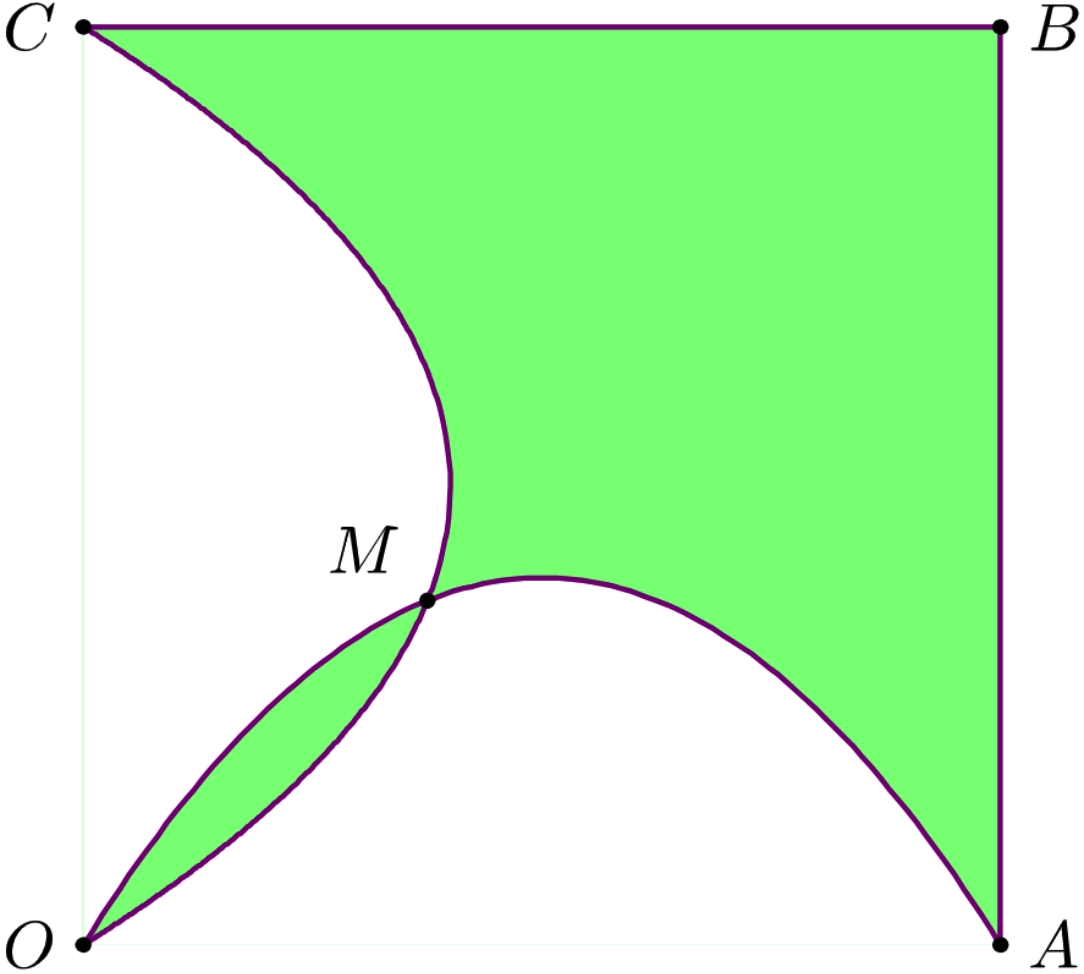
\includegraphics[width=1\linewidth]{images/Ứng dụng tích phân/NBK-4.png}
    \end{wrapfigure}

    Bạn Tá Selu làm một chiếc diều từ 4 thanh tre gồm 2 thanh thẳng cùng dài $80$cm, hai thanh còn lại được uốn cong thành hai đường parabol $(P_1)$ và $(P_2)$. Bạn Tá Selu cố định 4 thanh tre trên tại 5 vị trí $A$, $B$, $C$, $M$, $O$ sao cho $OABC$ là một hình vuông, sau đó dán giấy màu để tạo thành chiếc diều (tham khảo hình vẽ).Tính diện tích phần giấy màu bạn Đặng Cao Bồ cần cắt để giúp bạn Tá Selu tạo thành chiếc diều (đơn vị $cm^2$), biết rằng điểm $M$ cách đều hai đoạn thẳng $AB$ và $BC$ một khoảng bằng $50$cm. \textit{(làm tròn kết quả đến hàng đơn vị)}
}
\begin{minipage}{0.65\textwidth}
    Ta có: $
        \begin{cases}
            O(0;\,0),\; A(80;\,0),\; M(30;\,30) \in (P_1) \\
            O(0;\,0),\; C(0;\,80),\; M(30;\,30) \in (P_2)
        \end{cases}$\par
    $\Rightarrow
        \left\{\begin{aligned}
             & (P_1): y = -\dfrac{1}{50}x^2 + \dfrac{8}{5}x \\
             & (P_2): x = -\dfrac{1}{50}y^2 + \dfrac{8}{5}y
        \end{aligned}\right.$\par
    $\Rightarrow (P_2): \left\{\begin{aligned}
             & y = \dfrac{-1.6 + \sqrt{1.6^2 - 4\cdot 0.02x}}{-2\cdot 0.02}                 \\
             & y = \dfrac{-1.6 - \sqrt{1.6^2 - 4\cdot 0.02x}}{-2\cdot 0.02} < 0\, \forall x
        \end{aligned}\right.$\par
    $\Rightarrow S_1 = \displaystyle \int_{0}^{30}\dfrac{-1.6 + \sqrt{1.6^2 - 4\cdot 0.02x}}{-2\cdot 0.02} dx + \displaystyle \int_{30}^{80}(-\dfrac{1}{50}x^2 + \dfrac{8}{5}x)dx$\par
    $\Rightarrow S = 80^2 - 2S_1 = \dfrac{10040}{3} \approx \result{$3347\,cm^2$}$
\end{minipage}
\begin{minipage}{0.25\textwidth}
    \begin{figure}[H]
        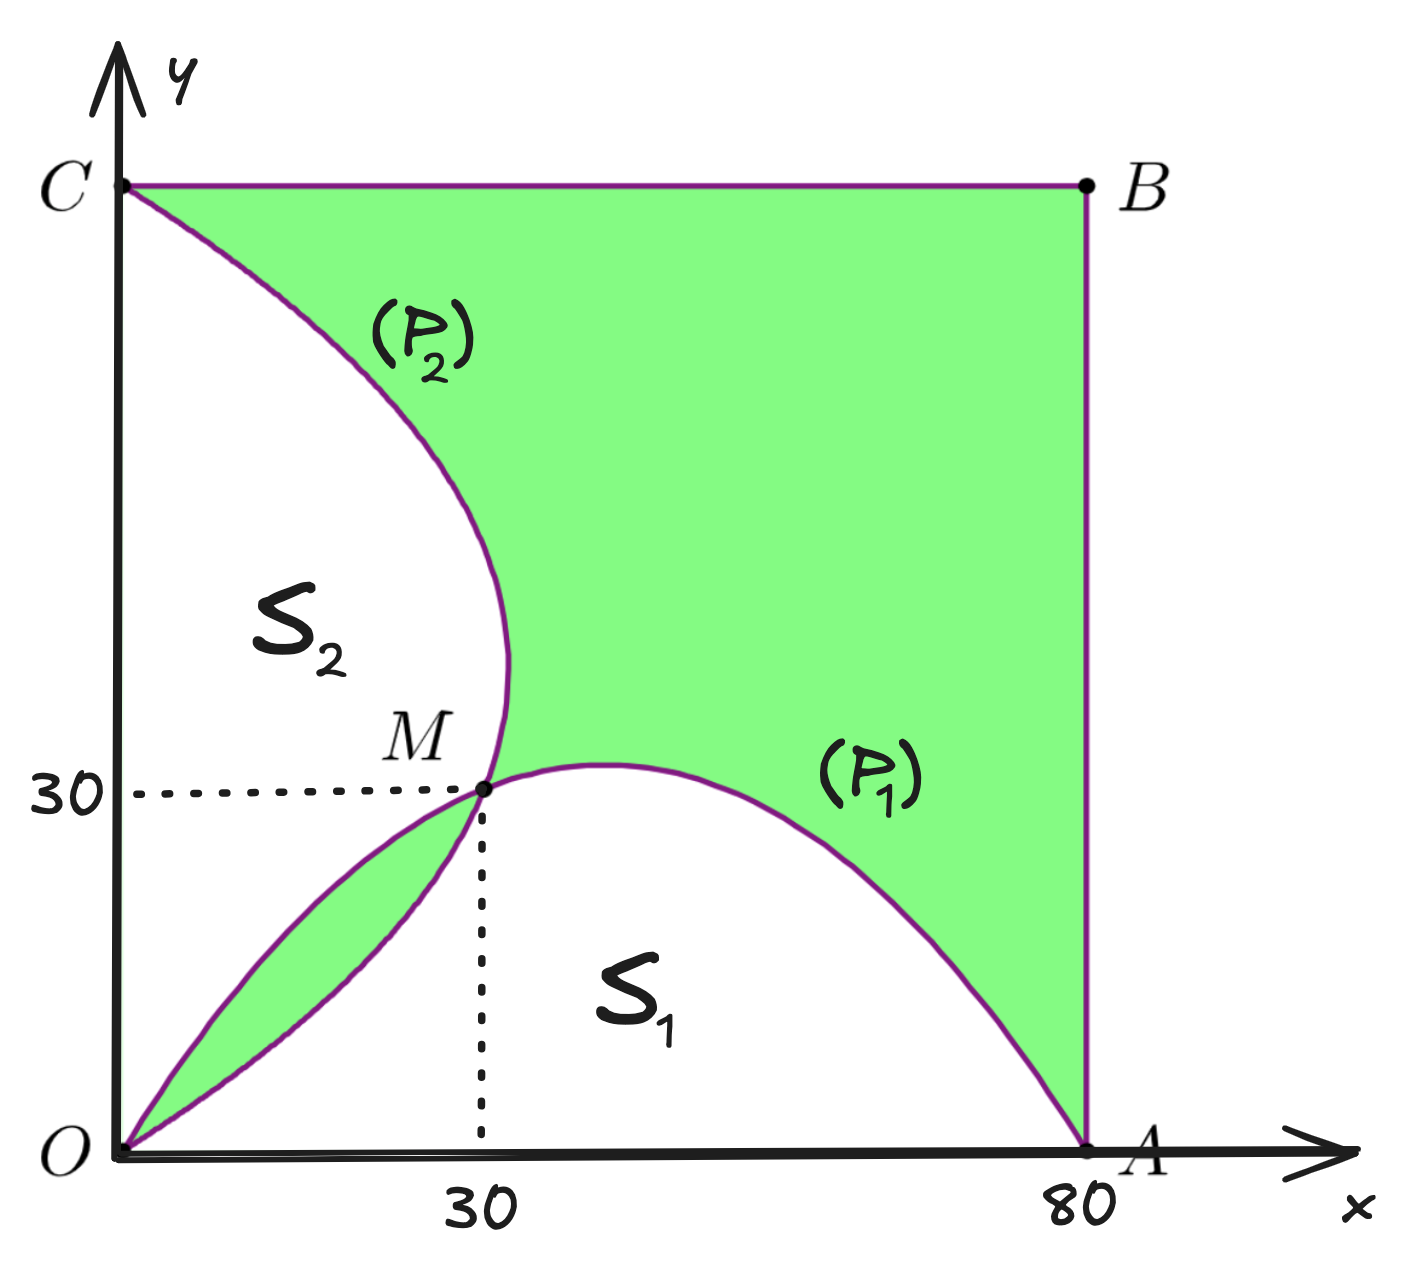
\includegraphics[width=1.5\textwidth]{images/Ứng dụng tích phân/NBK-4-solve.png}
    \end{figure}
\end{minipage}
\newpage\section{Toán rời rạc}
\exercise{
    \textcolor{red}{\textit{2425 -- Nguyễn Khuyến - Lê Thánh Tông}}

    Có 3 phương tiện chuyển động cùng hướng trên một đại lộ theo 3 đường thẳng song song được biểu diễn trên một mặt phẳng:
    \begin{itemize}[itemsep=0pt, topsep=0pt, parsep=0pt,label=--]
        \item Một ô tô con (xem như điểm $A$) chuyển động trên đường thẳng $d_1$ với tốc độ không đổi $20m/s$.
        \item Một xe container (xem như đoạn thẳng $EF$) dài $20$m ($EF=20$m) chuyển động với tốc độ không đổi $16m/s$ trên đường thẳng $d_2$ song song và cách $d_1$ một khoảng $10$m.
        \item Một xe cảnh sát (xem như điểm $P$) chuyển động với tốc độ không đổi $16m/s$ trên đường thẳng $d_3$ song song và cách $d_2$ một khoảng $10$m.
    \end{itemize}

    Phát hiện ô tô con có dấu hiệu vi phạm an toàn giao thông, xe cảnh sát tăng tốc với tốc độ $v(t) = 16 + \dfrac{t}{2} (m/s)$ để đuổi theo ô tô con, với $t$ (giây) là khoảng thời gian tính từ lúc bắt đầu tăng tốc. Tại thời điểm tăng tốc, xe cảnh sát cách ô tô con $50$m (dọc theo chiều đại lộ) và cách đuôi xe container (điểm $F$) $150$m (dọc theo chiều đại lộ). \textit{(tham khảo hình vẽ)}

    \begin{figure}[H]
        \centering
        \includegraphics*[width=0.55\textwidth]{images/Toán rời rạc/NK.png}
    \end{figure}

    Trong thời gian xe cảnh sát tăng tốc, ô tô con và xe container vẫn duy trì tốc độ như trên đồng thời các xe không thay đổi quỹ đạo chuyển động. Sau khi tăng tốc được $28$ giây thì xe cảnh sát bắt đầu giảm tốc để xử lý tình huống.

    Trong khoảng thời gian xe cảnh sát tăng tốc, xe container che khuất tầm nhìn của xe cảnh sát đối với xe ô tô con (nghĩa là hai đoạn thẳng $AP$ và $EF$ có điểm chung) trong khoảng thời gian bao lâu? \textit{(làm tròn kết quả đến hàng phần chục)}
}
\end{document}